% This is LLNCS.DEM the demonstration file of
% the LaTeX macro package from Springer-Verlag
% for Lecture Notes in Computer Science,
% version 2.4 for LaTeX2e as of 16. April 2010
%
\documentclass{llncs}
%
\usepackage{makeidx}  % allows for indexgeneration
\usepackage{graphicx}
\usepackage[sort&compress]{natbib}
%
\begin{document}
%
\title{Purchase Prediction via Machine Learning in Mobile Commerce}
%
\maketitle
%
\begin{abstract}
In the advent of the information era, electronic commerce has
developed rapidly and has become significant for every business.
Recommender systems play an essential role in it,
with the goal to aid users in buying items
fitting their taste from an overwhelming set of choices.
In this paper, we propose a machine learning approach
for a purchase prediction task launched by the Alibaba Group
based on the intuition that users' purchase behaviors
will be influenced by their historical browsing behaviors.
In our approach, this purchase prediction task is treated as
a binary classification problem
and five kinds of features are explored to learn potential model
of the influence of historical browsing behaviors,
including user quality, item quality, category quality,
user-item interaction and user-category interaction.
Because of the special nature of the mobile platform,
time factor and spacial factor are considered specially.
We incorporate time factor into the feature families
and extracte features in different time dimension.
Meanwhile, if the location of items is far away from users' site,
we think that purchase behaviors will not happen between them
according to the spacial factor.
\keywords{Recommender System, Purchase Prediction, Machine Learning}
\end{abstract}
%
\section{Introduction}
With the rapid growth of electronic commerce,
recommender systems are widely used to recommend items that fit the user's taste
to aid user in buying items from an overwhelming set of choices.
The goal of recommender systems is to help identify user preferences over items and
reflect the relationship between users and items \cite{lu2012recommender}.
Traditional methods in recommender systems are usually based on
CF (Collaborative Filtering),
in which the similarity of users and items are considered.
In addition, some methods take advantage of the users' historical behaviors
to extract their potential interests,
such as browsing click-stream, purchase time and frequency.

Recently, the Alibaba Group launched a purchase prediction task known as
Ali Mobile Recommendation Algorithm \footnote{http://tianchi.aliyun.com}.
This purchase prediction task provides the historical behaviors data of users
in the mobile platform during a period of one month
to help predict purchase behaviors will happen in the following ``one'' day.
The goal of this purchase prediction task is a little different from recommender system.
For example, if we recommend a item to one user and he likes it very much,
but he buys it a week later instead of in that day because of lack of money.
Then, this recommendation is a good case in recommender system
but a bad one in this purchase prediction task.
The differnece means that this purchase prediction
task cares more about the time factor.
Meanwhile, this task is based on
a typical O2O (Online to Offline) business model,
in which users pay online and consume offline.
It's almost impossible that a user in China buy a cinema ticket online,
and consume it offline in the cinema in America.
Hence, the spacial factor also plays an importance role in this task.

In this paper,
we propose a machine learning approach to solve this purchase prediction task,
instead of CF-based methods.
This task is treated as a binary classification problem,
and five kinds of features are explored from differnet aspects
to learn potential model of the historical browsing behaviors,a
including user quality, item quality, category quality,
user-item interaction and user-category interaction.
Those features could reflect the willing of users to buy items.
In particular, we focus on the time and spacial factor according to previous analysis.
The time factor is incorporated into the feature families
and features are extracted in different time dimension.
The spacial factor is used in the filter module.
For any purchase behaviors we predict, if the location of item
is far away from the user, we will remove it from our prediction results.

The remainder of the paper is organized as follows.
In section 2, we first discuss related work
in recommender systems and purchase prediction.
In section 3, we define the definition of
this purchase prediction task launched by the Alibaba Group.
Section 4 introduces the detail of the machine learning approach we propose.
Experiments and results are demonstrated to evaluate the efficiency
and effectiveness of the proposed approach in section 5.
Section 6 provides conclusions and outlines futures research directions.


\section{Related Work}
The most prominent technique in recommender system is
Collaborative Filtering (CF) \cite{su2009survey}.
The basic insight for this technique is a sort of continuity in the realm of taste.
If users Alice and Bob have the same utility for items $1$ through $k$,
then the chances are good that they will have the same utility for item $k + 1$.
Usually, these utilities are based on ratings that users have supplied for items
with which they are already familiar.
CF is roughly classified into two categories,
i.e. memory-based approachs \cite{linden2003amazon, wang2006unifying}
and model-based approachs \cite{adomavicius2005toward, koren2009matrix}.

The Netflix nillion-dollar challenge boosted interset in CF and yielded
the publication of a number of new methods.
Several matrix factorization techniques have been successfully applied to CF,
including Singular Value Decomposition (SVD) \cite{paterek2007improving}
and Non-negative Matrix Factorization (NMF) \cite{lee1999learning}.
A joint non-nagative matrix factorization method proposed in \cite{ju2014modeling} 
trys to solve the purchase prediction task launched by the Alibaba Group in 2014.
The goal of that task in 2014 is to predict purchase behaviors in the following one month
based on historical behaviors data in a period of four months.


\section{Problem Definition}
In many cases we need to develop an individualized recommendation system
for a subset of all items. When fulfilling such task,
besides utilizing the user behaviors data
in such subset of items, we also need to utilize
more comprehensive user behaviors data.
Notations:
\begin{itemize}
	\item $U$ stands for the set of users
	\item $I$ stands for the whole set of items
	\item $P$ stands for the subset of items, $P \subseteq I$
	\item $D$ stands for the user behaviors data set in all the set of all items
\end{itemize}

Our objective is to develop a recommendation model
for users in $U$ on the business domain $P$ using the data $D$.
In detail, our goal is to predict purchase behaviors over $P$
in the following one day based on the behaviors data during one month in $D$.


\section{Method}
The target of the purchase prediction task is to predict purchase behaviors will happen
in the following one day based on the historical behaviors in the last month.
We treat the target problem as a binary classification problem,
i.e. any ($user$, $item$) pairs will be divided into two classes:
``buy'' and ``not buy''.
We propose a machine learning approach to solve this task,
the framework of which is showed in Figure \ref{fig:framework}.

\begin{figure}[htbp]
	\centering
	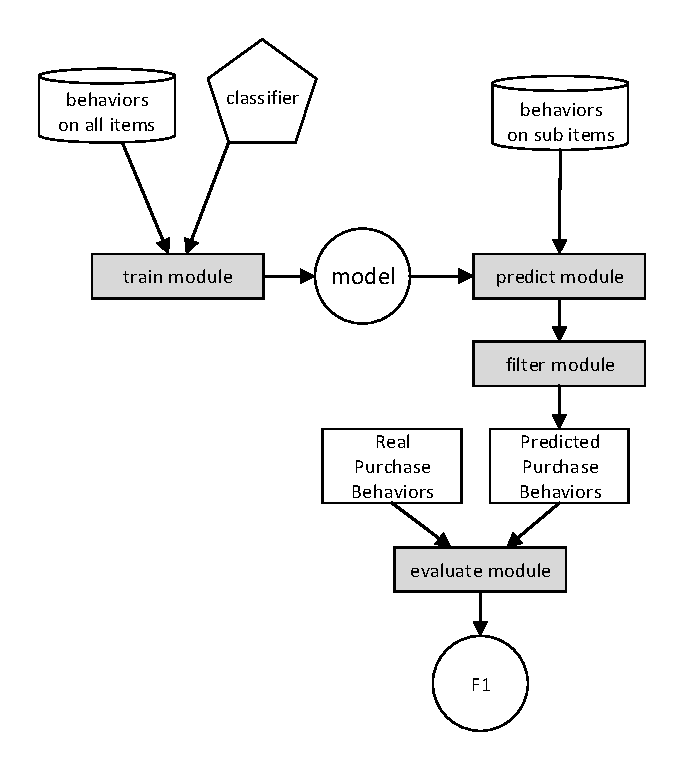
\includegraphics[scale=0.6]{images/system.pdf}
	\caption{Machine Learning Framework}
	\label{fig:framework}
\end{figure}

First, we would like to learn a model from
the behaviors data over the whole set of items in the \textbf{train module},
which can reflect why users will buy items in the following one day
and how their historical behaviors influence their future purchase behaviors.
In detail, if $user$ buy $item$ in the following one day,
this ($user$, $item$) pair will be labeled as a positive instance
while other pairs that doesn't be bought
are going to be labeled as a negative instance.
In addition, this trained model is applied to the behaviors data over
the subset of items in the \textbf{predict module}
and positive instances in the prediction results will be seen as
purchase behaviors will be happen in the following one day.
Then, we take spacial factor into consideration and remove pairs
with too long distance in those positive instances
via the \textbf{filter module}.
In the last, the filtered predicted purchase behaviors are
compared with the real purchase behaviors to evaluate
the performance of our approach in the \textbf{evaluate module}.

\subsection{Train Module and Predict Module}
Training set is a base component in the train module just like
test set in the predict module,
but there is a little difference between the generation of them.
Because we cann't use the future infomation,
i.e. we don't know purchase behaviors
on the whole set of items in the following one day,
we split baheviors data in the lastday of the month
and use them to label ($user$, $item$) pairs that appear
in the remainder of the month.
This process is illustrated in Figure \ref{fig:train_and_test}.

\begin{figure}[htbp]
	\centering
	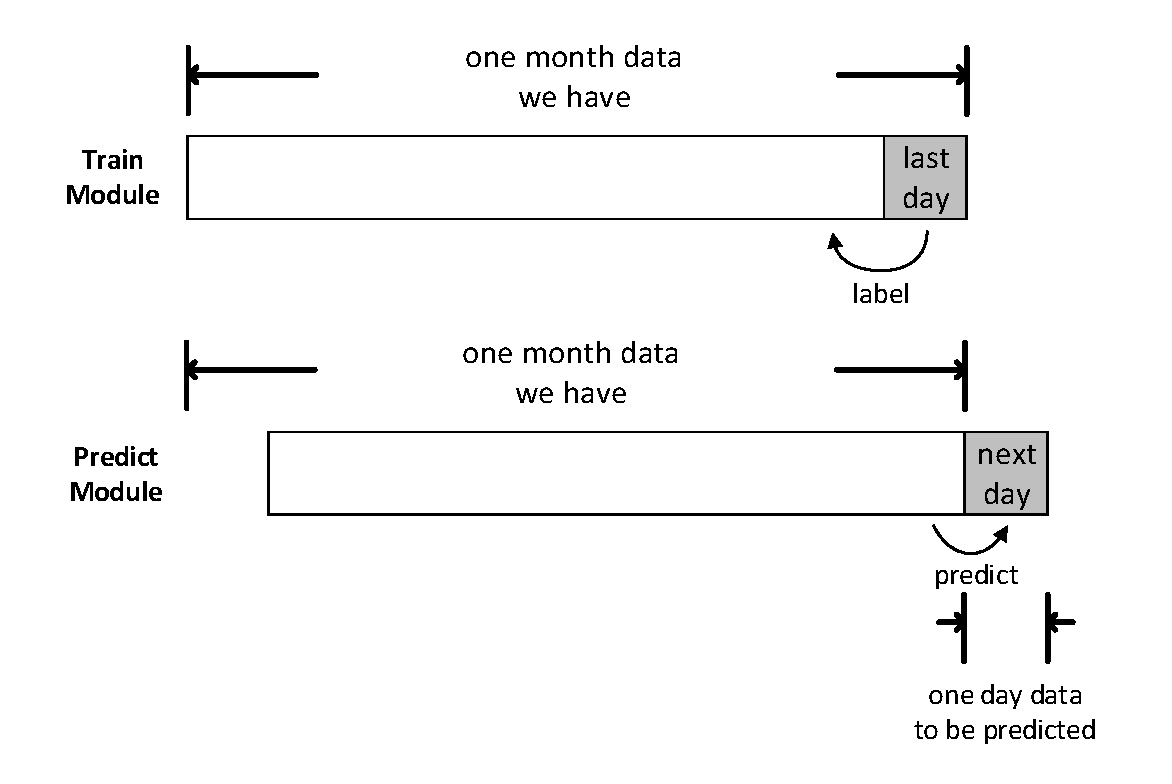
\includegraphics[scale=0.4]{images/train_and_test.pdf}
	\caption{Training Set and Test Set}
	\label{fig:train_and_test}
\end{figure}

\subsection{Feature Project}
Feature project is an important component in our machine learning approach
and we will discuss feature families detailly in this section.

For a certain ($user$, $item$) pair, the $item$ belongs to a $category$,
we consider the following five feature families,
i.e. user quality, item quality, category quality, user-item interaction
and user-category interaction.

\textbf{User Quality} estimates the purchasing power and vitality of users.
In the mobile commerce, some users are active and have strong purchase desire
while others are inactive and not willing to buy items frequently.

\begin{itemize}
	\item \emph{Last Login Day} represents the last login day of a user.
	If a user's last login day is close to the following one day
	we think that this user is active recently
	and he has a strong possibility to login in the following one day.
	
	\item \emph{Conversion Ratio} represents the ratio of purchase behaviors of a user
	in his total behaviors. High Conversion Ratio means this user
	has a strong purchasing power.
	
	\item \emph{Behaviors Statistics} stands for the count of a user's behaviors.
	The more this user browse, the higher possibility he will buy.
	There is an example in the left of Figure \ref{fig:active} to explain the definition.
	In this example, a user click for $3$ times in the first day, $1$ time in the second day and
	$2$ times in the fourth day, so the count of his total behaviors in the last four day equals
	$3 + 1 + 0 + 2 = 6$.
	
	\item \emph{Active Days} means the count of active days of a user.
	This feature could represent the positivity of a user directly.
	There is an example in the right of Figure \ref{fig:active} to explain the definition.
	In this example, a user login in the first day, the second day and
	the fourth day, so the count of his active days in the last four day equals
	$1 + 1 + 0 + 1 = 3$.
	
\end{itemize}

\begin{figure}[htbp]
	\centering
	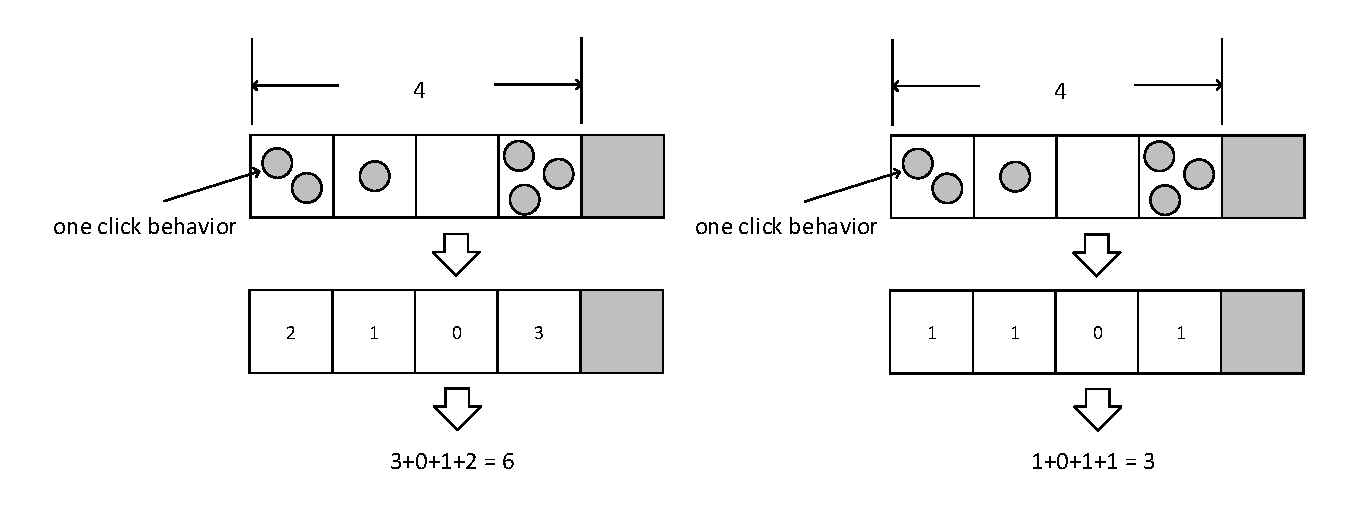
\includegraphics[scale=0.5]{images/active.pdf}
	\caption{An Example of Behaviors Statistics}
	\label{fig:active}
\end{figure}

\textbf{Item Quality} reflects the popularity of a item.
Obviously, more popular items have bigger tendency to be bought.
\begin{itemize}
	\item \emph{Last Browsed Day} represents the last day a item is browsed.
	If a item's last browsed day is close to the following one day
	we think that this item is active recently
	and it has a strong possibility to be browsed in the following one day again.
	
	\item \emph{Conversion Ratio} represents the ratio of purchase behaviors of a item
	in its total browsed behaviors. High Conversion Ratio means that users usually buy it
	with a small number of click and this item is worth to be bought.
	
	\item \emph{Behaviors Statistics} stands for the count of a item's browsed behaviors.
	The more this item is browsed, the higher possibility it will be bought.
	
	\item \emph{Active Days} means the count of days a item is browsed.
	This feature could represent the popularity of a item.
\end{itemize}

\textbf{Category Quality} describes the popularity of a category.
The definition of \emph{Last Browsed Day}, \emph{Conversion Ratio},
\emph{Behaviors Statistics} and \emph{Active Days} in it is similar
with those in \textbf{Item Quality}.

\textbf{User-Item Interaction} describes the interaction between the user and item.
it is a direct aspect to reflect the willing that the user want to buy the item.
\begin{itemize}
	\item \emph{Behaviors Statistics} represents the count of a user's browsing behaviors on one item.
	It's obvious that if a user is interested in one item and willing to buy it,
	he will browse it frequently to know it completely in recent days.
	
	\item \emph{Active Days} means the count of days in which the user browse the item.
	The more active days, the user is more active and has a bigger willing to buy the item.
\end{itemize}

\textbf{User-Category Interaction} represents the interaction between the user and the category.
It is similar with \textbf{User-Item Interaction},
and \emph{behaviors Statistics} and \emph{Active Days} will be generated in the same way.

\subsection{Filter Module}
This purchase prediction task is based on a typical O2O business model,
in which users pay online and consume offline.
This means that users are not willing to buy items
which is far away from them because they have to
go there to consume.
Based on the fact, we propose Filter Module to
remove those pairs with too long distance.
In detail,
in a ($user$, $item$) pair,
if the distance between the location of the $item$ and the $user$ is bigger than $L$,
any purchase behaviors will happen on this pair.
We set $L = 100km$ from experience in this paper.

\subsection{Classifier}
Three classifier are considered in our machine learning approach,
including LR (Linear Regression), RF (Random Forest) and GBDT (Gradient Boosting Decision Tree).

In Linear Regression, data are modeled using linear predictor functions,
and unknown model parameters are estimated from the data.
Most commonly, linear regression refers to a model
in which the conditional mean of y given the value of X
is an affine function of X.

Random Forest \cite{breiman2001random} is an ensemble learning method
for classification, regression and other tasks,
that operate by constructing a multitude of decision trees at training time and
outputting the class that is the mode of the classes (classification)
or mean prediction (regression) of the individual trees.
Random forests correct for decision trees' habit of overfitting to their training set.

Gradient boosting is a machine learning technique for regression and classification problems,
which produces a prediction model in the form of an ensemble of weak prediction models,
typically decision trees \cite{friedman2003multiple}.
It builds the model in a stage-wise fashion like other boosting methods do,
and it generalizes them by allowing optimization of an arbitrary differentiable loss function.

\begin{table}[htbp]
	\normalsize
	\centering
	\caption{The Comparison of Three Classifiers}
	\begin{tabular}{|c|c|c|}
		\hline
		\textbf{Classifier} & \textbf{Speed} & \textbf{Performance} \\
		\hline
		LR & quick & poor \\
		\hline
		RF & middle & middle \\
		\hline
		GBDT & slow & good \\
		\hline
	\end{tabular}
	\label{tab:comparison}
\end{table}

The comparison of those classifiers is showed in Table \ref{tab:comparison}.
We can see from that LR is simple and can train and predict in a very short period of time,
but the performance of it is poor.
GBDT need lots of time to train and predict and its performance is best of them.
The speed and performance of RF is between LR and GBDT. 

\subsection{Reduced Data}
Because the volume of out data set is too large,
it will spend unacceptable time for training process
in the machine learning approach.
Hence, we use a reduced data set to solve this problem
and keep prediction performance at the same time,
which is showed in Figure \ref{fig:reduced_data_set}.

\begin{figure}[htbp]
	\centering
	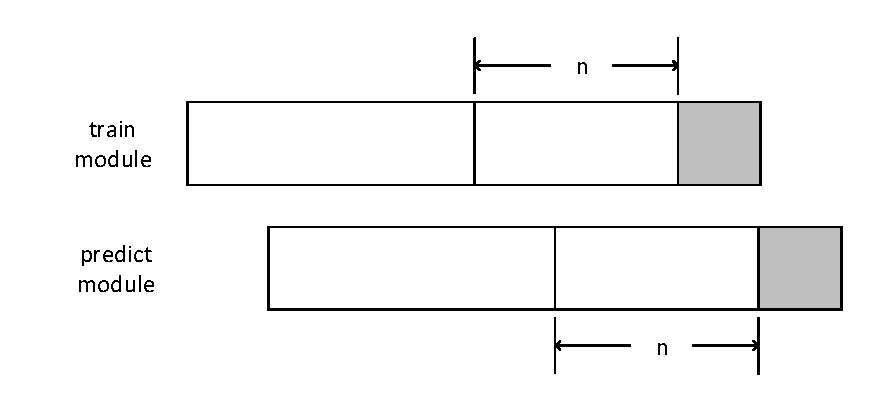
\includegraphics[scale=0.5]{images/reduced_data_set.pdf}
	\caption{Definition of the Reduced Data Set}
	\label{fig:reduced_data_set}
\end{figure}

Instead of using all the ($user$, $item$) pairs happened in the one month,
we use pairs show up in last $n$ days to train and predict.
$n = 1$ means that we use data in the last day while
$n = 30$ means that we use all data over the whole one month.

\subsection{Negative Sampling}
The positive instances and negative instances are not balanced in the training set,
the count of negative instances is far greater than that of positive ones.
If we use all of the data to train a model,
this model will prefer to judging all the inputs negative.
To handle this issue, we use classic \textbf{Negative Sampling} method,
i.e. we use part of negative instances instead of all of the negative ones,
just like \cite{bowling2006machine}.

\section{Experiments}
\subsection{Data Description}
The data contains two parts.
The first part is the dataset $D$, the mobile behaviors data of users in the set of all items,
with the following columns:
\begin{itemize}
	\item $user\_id$ : identity of users
	\item $item\_id$ : identity of items
	\item $behaviors\_type$ : the user behaviors type, including click, collect, cart and buy
	\item $user\_geohash$ : user location when the behaviors occurs, which may be null
	\item $item\_category$ : the category id of the item
	\item $time$ : the time of the behaviors, which is converted to the nearest hours
\end{itemize}

The second part is the dataset $P$, the subset of items data,
with the following columns:
\begin{itemize}
	\item $item\_id$ : identity of items
	\item $item\_geohash$ : item location, which may be null
	\item $item\_category$ : the category id of the item
\end{itemize}

The training data contains the mobile behaviors data of
certain quantity of sampled users ($D$) from November 18, 2014
to December 18, 2014.
The evaluation data is the purchase data of these same users of
the items in $P$ in December 19, 2014.
We should develop a model from behaviors data in a month
to predict the purchase behaviors of the users of the items
in the following one day.

Summary statistics of the data are listed in Table \ref{tab:sta}.
\begin{table}[htbp]
	\normalsize
	\centering
	\caption{The Statistics of The Data Set}
	\begin{tabular}{|c|c|c|c|c|c|}
		\hline
		\#table $D$ & \#table $P$ & \#user set & \#total item set & \#sub item set & \#category set \\
		\hline
		5,822,532,780 & 14,397,493 & 5,000,000 & 156,226,243 & 13,435,163 & 13,128 \\
		\hline
	\end{tabular}
	\label{tab:sta}
\end{table}

\subsection{Metrics}
We use Precision, Recall and F1 scores as the evaluation metric, which are defined as follows:

$$ Precision = \frac{ \left| PredictionSet \cap ReferenceSet \right| }{ \left| PredictionSet \right| } $$
$$ Recall = \frac{ \left| PredictionSet \cap ReferenceSet \right| }{ \left| ReferenceSet \right| } $$
$$ F1 = \frac{ 2 \times Precision \times Recall }{ Precision + Recall } $$

Where, $PredictionSet$ contains the predict purchase data and $ReferenceSet$ contains the real purchase data.
We take F1 score as the only standard of the final evaluation.

\subsection{Two Rule-Based Baseline}
\emph{CartRule} is the first strategy of most partipants, and we select it as our first baseline.
In detail, \emph{CartRule} thinks that if a user add a item into his cart and doesn't buy it in that day,
it's likely that he will buy it in the next day.

In addition, we add time factor into consideration based on \emph{CartRule}
and propose \emph{CartRule2}.
\emph{CartRule2} thinks that if a user add a item into his cart and doesn't buy it
after $m$ o'clock ($ m \in \{ 0, 1, ..., 23 \} $) in that day,
it's likely that he will buy it in the next day.

\begin{figure}[htbp]
	\centering
	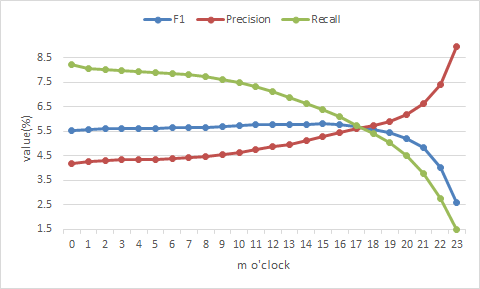
\includegraphics[scale=0.6]{images/rule.png}
	\caption{Performance of Different $m$ in CartRule2}
	\label{fig:rule}
\end{figure}

Figure \ref{fig:rule} shows the performance of those methods using different $m$.
We can see from that,
The precision is increasing while the recall is decreasing
with the increase of $m$ and less pairs are returned.
In addition, the F1-score increases before $15$ o'clock slowly
and decreases after $15$ o'clock.

\subsection{Result}
\begin{table}[htbp]
	\normalsize
	\centering
	\caption{Performance of Different approachs}
	\begin{tabular}{|p{60pt}|p{60pt}|p{60pt}|p{60pt}|}
		\hline
		Approach & F1(\%) & Precision(\%) & Recall(\%) \\
		\hline
		CartRule & 5.5480 & 4.1824 & 8.2377 \\
		CartRule2 & 5.8007 & 5.3018 & 6.4033 \\
		\hline
		n1\_LR & 6.8985 & 7.8298 & 6.1652 \\
		n1\_RF & 8.0064 & 8.3249 & 7.7114 \\
		n1\_GBDT & \textbf{8.3841} & \textbf{8.2591} & \textbf{8.5129} \\
		\hline
		n2\_LR & 6.3266 & 6.5820 & 6.0902 \\
		n2\_RF & 7.9830 & 8.5378 & 7.4959 \\
		n2\_GBDT & \textbf{8.4264} & \textbf{8.2036} & \textbf{8.6617} \\
		\hline
		n3\_LR & 6.5542 & 7.4360 & 5.8593 \\
		n3\_RF & 7.9152 & 8.9481 & 7.0960 \\
		n3\_GBDT & \textbf{8.4719} & \textbf{8.6591} & \textbf{8.2926} \\
		\hline
		n4\_LR & 6.5015 & 7.1628 & 5.9520 \\
		n4\_RF & 7.9152 & 8.8237 & 7.1764 \\
		n4\_GBDT & \textbf{8.4410} & \textbf{8.4336} & \textbf{8.4485} \\
		\hline
	\end{tabular}
	\label{tab:score}
\end{table}

We set $n \in \{ 1, 2, 3, 4\}$ in the reduced data in this paper
and apply three classifiers (LR, RF and GBDT) on them.
Table \ref{tab:score} shows the prediction performance of different approachs
in this purchase prediction task.
`n1\_LR' means that $n = 1$ and $classifier = LR$,
`n4\_GBDT' means that $n = 4$ and $classifier = GBDT$,
others could be explainedn in the same way.

$CartRule2$ has a little improvement compared to $CartRule$
because $CartRule2$ takes the time factor into consideration.
Those machine learning approachs we proposed have a much better performance
than two rule-based methods, which could proves the effectiveness of our approachs to some extent.
Compare the performance of different classifiers,
we could see easily that $GBDT$ is the best choice.
With the increase of $n$, the F1-score changes littlely.
This phenomenon proves that reduced data could accelerate
the process of machine learning and keep the performance at the same time.

\begin{table}[htbp]
	\normalsize
	\centering
	\caption{Performance of Different Features}
	\begin{tabular}{|p{66pt}|p{60pt}|p{60pt}|p{60pt}|}
		\hline
		Approach & F1(\%) & Precision(\%) & Recall(\%) \\
		\hline
		U & 0.3429 & 5.8870 & 0.1766 \\
		I & 0.9405 & 6.6290 & 0.5061 \\
		C & 0.0000 & 0.0000 & 0.0000 \\
		UI & 6.6802 & 8.2817 & 5.5977 \\
		UC & 2.1693 & 6.7042 & 1.2940 \\
		\hline
		U + I + C & 2.8068 & 7.3183 & 1.7364 \\
		UI + UC & 7.4938 & 8.2366 & 6.8740 \\
		\hline
		All(n3\_GBDT) & 8.4719 & 8.6591 & 8.2926 \\
		\hline
	\end{tabular}
	\label{tab:fea}
\end{table}

To prove the effectiveness and robustness of feature families explored,
we test a series of combination of feature families on 
``n3\_GBDT'', which is the best result mentioned above.
First, we try to use one of five kinds of features only to predict.
`U' means using User Quality features only,
`I' means using Item Quality features only,
and so on.
Then, we use individual features, i.e.
User Quality, Item Quality and Category Quality,
to test purchase behaviors between active users and popular items,
which is represented as `U + I + C'.
At the last, we ignore the quality of users and items,
just use the interaction between them (`UI + UC') to predict.
`All' means five kinds of features will be used totally.
The prediction performance of different strategies is demonstrated in Table \ref{tab:fea}.

The performance of `U', `I' and `C' is very poor while the performance of `UI' is middling,
which explains the importance of interaction features.
The count of purchase behaviors between active users and popular items is sensible
according to the performance of `U + I + C'.
Compare the performance of `UI + UC' and `UI', we can see that
category also has a strong influence on the purchase behaviors.
The performance of `All' is the best, which could prove the effectiveness and
robustness of feature families we explored to some extent.


\section{Conclusion}
Based on the intuition that the purchase behaviors of a user
will be affected with his history behaviors,
we present a machine learning approach to solve
the purchase prediction task launched by the Alibaba Group.
Five kinds of features are explored to descript
the willing of users' purchase desire on items.
In particular, we take the time and spacial factor into consideration.
Time factor is incorporated into the feature project while
spacial factor is used in the filter module.

Lots of work could be further studied in the future.
Many items are bought frequently such as cinema tickets
while others are bought for only once such as laptop.
Based this fact that the purchase frequency of items is different
we could treat the purchase prediction task
as four classification problem, i.e.
`not buy before and will not buy', `not buy before and will buy',
`buy before and will not buy' and `buy before and will buy'.
In addition, the way we use the time and spacial factor is simple,
we can also combine them and user quality
and build different prediction models for different type of users.

\bibliographystyle{abbrv}
\bibliography{llncs}
\end{document}
